\section{Real-time network model}
\label{sec:nw_realtime}

Due to the time constraints of real-time applications, our framework uses a Kalman filter to implement the model described above, which, as previously discussed, is a highly efficient estimation method. This requires the transition and measurement matrices as described in \cref{sec:kf} on \cpageref{sec:kf}. The measurement matrix is the identity matrix $\mat{I}$ since the data are direct observations of the underlying state (average vehicle speed),
\begin{equation}
\label{eq:kf_meas_identity}
\NWstate_{\ellc} = \mat{H}\Vttobs_{\ellc} + w_{\ellc} =
\Vttobs_{\ellc} + w_{\ellc},
\end{equation}
where the measurement error $w_{\ellc} \sim \Normal{0}{\NWvar_{\ell}^2 + \Vtterr_{\ellc}^2}$ consists of between-vehicle and observation errors, which are assumed to be independent. We also use the identity matrix for the transition matrix $\mat{F}$ as our best guess of the current traffic state is the previous state. So, assuming that $\NWvar_{\ell}$ and $\NWnoise_{\ell}$ are known, for now, we have everything needed to implement a Kalman filter on $\NWstate_{\ellc}$.


\subsection{Predict step}
\label{sec:kf_predict}

In the examples presented, we use a stationary transition function, that is, $\mat{F}_c = 1$, which implies an assumption that traffic speed is constant over short periods (less than five~minutes). The vector of all segment speed observations up to and including time $t_{c}$ is defined as
\begin{equation}\label{eq:all_seg_obs}
\NWobs_{\ell,1:c}^{\boldsymbol{\cdot}} = \bigcup_{t=1}^{c} \bigcup_{v\in V_{\ell,t}} \NWobs_{\ell,t}^v,
\end{equation}
where $V_{\ellc}$ is the set of all vehicles traversing segment $\ell$ at time $t_c$. Then the estimated segment state, conditional on all observations up to time $t_{c-1}$, has mean
\begin{equation}\label{eq:ch4:nw_state_mean_est}
\hat\NWstate_{\ellc|c-1} =
    \E{\NWstate_{\ellc} \cond{} \NWobs_{\ell,1:c-1}^{\boldsymbol{\cdot}}}
\end{equation}
and variance
\begin{equation}\label{eq:ch4:nw_state_var_est}
\NWstatevar_{\ellc|c-1} =
    \Var{\NWstate_{\ellc} \cond{} \NWobs_{\ell,1:c-1}^{\boldsymbol{\cdot}}},
\end{equation}
which are predicted using the following equations:
\begin{equation}
\label{eq:nw_kf_predict}
\begin{split}
\hat\NWstate_{\ellc|c-1} &=
    \hat\NWstate_{
\ellc-1|c-1}, \\
\NWstatevar_{\ellc|c-1} &= \NWstatevar_{\ellc-1|c-1} + \left(\NWtdiff_c\NWnoise_\ell\right)^2.
\end{split}
\end{equation}
This prediction is shown in \cref{fig:nw_kf1}. Alternatively, were forecast information available, we could use a transition matrix $\mat F_c$ to describe how traffic might change over time, as is shown in \cref{fig:nw_kf2}.


\begin{knitrout}\small
\definecolor{shadecolor}{rgb}{0.969, 0.969, 0.969}\color{fgcolor}\begin{figure}

{\centering \subfloat[Constant speed model. The prediction is equal to the previous state with an increased variance.\label{fig:nw_kf1}]{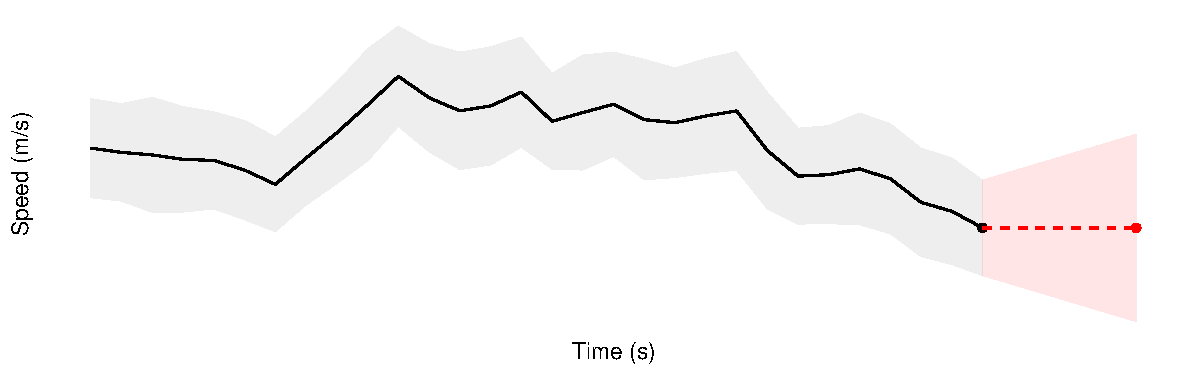
\includegraphics[width=0.8\textwidth]{figure/nw_kf-1} }\\
\subfloat[Historical change based model. The dashed blue line represents historical average speed, which the prediction accounts for under this model.\label{fig:nw_kf2}]{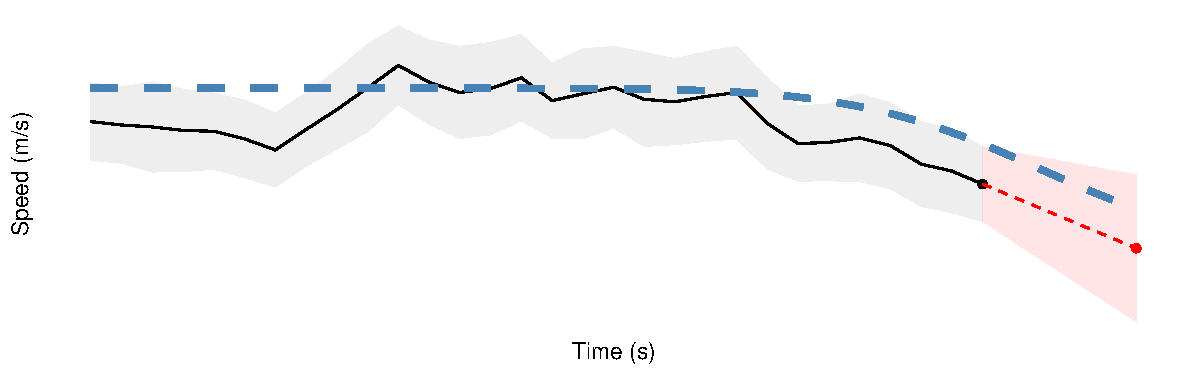
\includegraphics[width=0.8\textwidth]{figure/nw_kf-2} }\\

}

\caption[Network state prediction using constant speed and historical trend models]{Network state prediction depends solely upon the current state (black dot). The mean (solid black line) and uncertainty (shaded grey region) represent previous states. The predicted state has mean (red point) and uncertainty (shared pink region) dependent on the chosen model.}\label{fig:nw_kf}
\end{figure}


\end{knitrout}


\subsection{Update step}
\label{sec:kf_update}

Updating the \kf{} involves taking the predicted state and updating it using \emph{observations} of vehicle speeds along road segments. These are obtained from the \pf{} (\cref{sec:vehicle_speeds}). However, it is possible to have multiple observations per road segment in one update period, as it is common for buses to travel one behind the other, particularly along bus lanes. Therefore, we have an \emph{observation vector} for a set of vehicles $V_{\ellc}$ passing through segment $\ell$ in the time interval $(t_{c-1}, t_c]$.
% \begin{equation} \label{eq:nw_seg_obs}
% \NWobss_{\ell c} = \bigcup_{v\in V_{\ell c}} \Vttobs_{\ell c}^v,
% \end{equation}
% which can be the empty set $\NWobss_{\ell c} = \emptyset$ if no vehicles travel through the segment in the interval.


When updating the network, each observation must be accounted for. One way would be to combine the observations into a single estimate; however, this involves averaging observations and uncertainties. An alternative is to use an \emph{\infil{}}, which allows the summation of information from multiple observations \citep{Mutambara_2000}. The information filter involves inverting the state uncertainty $\NWstatevar$; however, this is a simple computation due to having a one-dimensional state---if we were to estimate the state of all segments simultaneously, inverting the $L\times L$ uncertainty matrix would be computationally demanding, or even impossible, and we would be unable to use the approach.



The first step converts the predicted state vector and covariance matrix into information space by inversion of the covariance matrix, leading to the information matrix
\begin{equation}\label{eq:nw_if_inf_matrix}
\NWinfmat_{\ellc|c-1} = \NWstatevar_{\ellc|c-1}^{-1}
\end{equation}
and information vector
\begin{equation}\label{eq:nw_if_inf_vector}
\NWinfvec_{\ellc|c-1} = \NWstatevar_{\ellc|c-1}^{-1} \hat\NWstate_{c|c-1}.
\end{equation}


Converting the observations into information follows the same formula. Note first that the error needs to account for both measurement error and between-vehicle variation, which are assumed Gaussian and independent, so the total variance is their sum. The observation information matrix is
\begin{equation}\label{eq:nw_if_inf_obsmatrix}
\NWobsinfmat_{\ellc}^v = \frac{1}{\NWvar_{\ell}^2 + (\NWerr_{\ellc}^v)^2}
\end{equation}
and the observation information vector is
\begin{equation}\label{eq:nw_if_inf_obsvector}
\NWobsinfvec_{\ellc}^v = \frac{\hat\NWobs_{\ellc}^v}{
    \NWvar_{\ell}^2 + (\NWerr_{\ellc}^v)^2
}.
\end{equation}
Combining these by summation over vehicles yields the complete information matrix and vector for the time period $(t_{c-1},t_c]$, which are, respectively,
\begin{equation}\label{eq:nw_if_obsupdate_matrix}
\NWobsinfmat_{\ellc} = \sum_{v\in V_{\ellc}} \NWobsinfmat_{\ellc}^v
\end{equation}
and
\begin{equation}\label{eq:nw_if_obsupdate_vector}
\NWobsinfvec_{\ellc} = \sum_{v \in V_{\ellc}} \NWobsinfvec_{\ellc}^v.
\end{equation}



The state update is now just a case of adding the observation information in \cref{eq:nw_if_inf_obsmatrix,eq:nw_if_inf_obsvector} to the predicted state information in \cref{eq:nw_if_inf_matrix,eq:nw_if_inf_vector}:
\begin{equation}
\label{eq:nw_if_update}
\begin{split}
\NWinfmat_{\ellc|c} &= \NWinfmat_{\ellc|c-1} + \NWobsinfmat_{\ellc}, \\
\NWinfvec_{\ellc|c} &= \NWinfvec_{\ellc|c-1} + \NWobsinfvec_{\ellc}.
\end{split}
\end{equation}
Note that, in situations where no data is observed for a given segment, the information for that segment is zero, so there is no further change to the predicted state value. This could be useful at peak hour, for example, if the transition function predicts changes based on historical trends.


Finally, we back-transform the information into the state space,
\begin{equation}
\label{eq:nw_if_statespace}
\begin{split}
\hat\NWstate_{\ellc|c} &= \NWinfmat_{\ellc|c}^{-1} \NWinfvec_{\ellc|c}, \\
\NWstatevar_{\ellc|c} &= \NWinfmat_{\ellc|c}^{-1}.
\end{split}
\end{equation}

The primary constraint on the model is the dependence on $\NWvar_{\ell}$ and $\NWnoise_{\ell}$; however, before considering the estimation of these values, we apply the Kalman filter model to the simulated data in \cref{fig:nw_sim_data} for which the parameter values are known.


\begin{knitrout}\small
\definecolor{shadecolor}{rgb}{0.969, 0.969, 0.969}\color{fgcolor}\begin{figure}

{\centering \subfloat[\kf{} estimate of the state mean (red line) and variance (shaded region) along with the true value (dashed black line).\label{fig:nw_simdata_fit-1}]{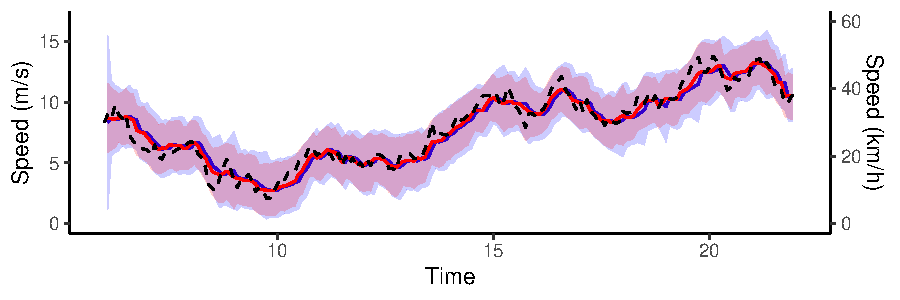
\includegraphics[width=.8\textwidth]{figure/nw_simdata_fit-1} }\\
\subfloat[Predictive distribution of average vehicle speed accounting for state uncertainty and between-vehicle uncertainty ($\NWvar^2$). Observations represented by black points.\label{fig:nw_simdata_fit-2}]{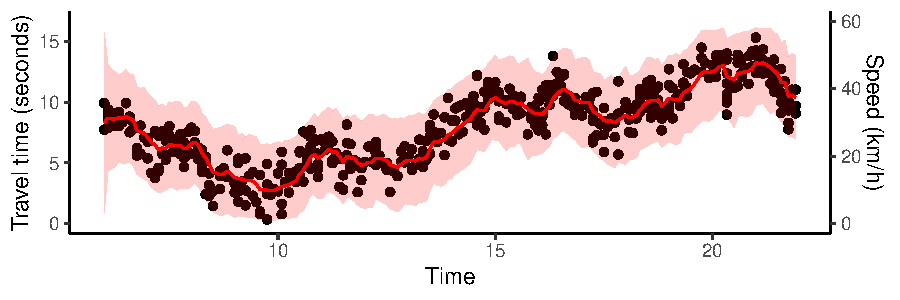
\includegraphics[width=.8\textwidth]{figure/nw_simdata_fit-2} }\\

}

\caption[Results of fitting the \kf{} to the simulated data]{Results of fitting the \kf{} to the simulated data.}\label{fig:nw_simdata_fit}
\end{figure}


\end{knitrout}

The \kf{} was fitted to the simulated data using the same values of $\NWnoise_\ell$ and $\NWvar_\ell$ used to generate the data, with the estimate of $\NWstate_{\ell,1:c}$ shown by the solid red line in \cref{fig:nw_simdata_fit-1} along with the associated uncertainty as estimated by $\NWstatevar_{\ell,1:c}$ (shaded region). A dashed black line represents the simulated true mean. We see that the 95\% credible region contains the true values of $\NWstate_{\ell,1:c}$. \Cref{fig:nw_simdata_fit-2} shows the posterior estimate of $\NWstate_{\ell,1:c}$ along with the posterior predictive distribution of $\NWobs_{\ellc}^m$; that is, using the 95\% region defined by the sum of $\NWstatevar_{\ell,1:c}$ and $\NWvar_\ell^2$, the latter of which is known for the simulation. Approximately 99.8\% of the observations lie within the 95\% predictive region. Given the network parameters $\NWnoise_\ell$ and $\NWvar_\ell$ are known, the underlying network state can be recovered using a \kf{}.


\subsection{Limitations of the implementations}
\label{sec:kf-limits}

The main limitation of using the information filter is the need to calculate the inverse of the covariance matrix. If we want to improve the model by including segment interactions, the dimensionality of $\NWstatevar$ would quickly become too large to compute $\NWstatevar^{-1}$ easily. Thus, the method presented here is only appropriate for independent segments. Fortunately, however, using the \kf{} instead would not be too difficult a task, since most of the time, only one vehicle will pass through a segment during an iteration. In cases where there is more than one, the estimates and their errors could be combined using a sample mean and variance, for example.
